\section{数据挖掘结果与认知边界}

在完成采集与预处理后，本文不只计算总体准确率，而是把每条模型回复看作一条行为记录，从描述层级、无关扰动、重复采样、错误文本和模型画像五个方向进行挖掘。当前版本包含 10{,}585 条成功模型回复，覆盖 9 个有成功样本的模型和 824 个唯一 \code{prompt_uid}。整体准确率为 45.5\%，其中 33.0\% 的回复被解析为 \code{uncertain}，说明模型面对轮椅转弯问题时经常不是简单答错，而是退回到“缺少信息、无法判断”的保守状态。

本节的核心发现可以概括为四点，如图 \ref{fig:key-findings-summary} 所示。第一，描述层级不是单向增益：有的模型在 L3 形式化表达下明显提升，有的模型反而发生数学化坍塌。第二，无关背景信息并非“无害噪声”，情绪压力、光照和材质颜色能够在几何参数不变时改变模型最终判断。第三，重复采样揭示了比随机波动更隐蔽的风险，即部分模型会稳定输出同一个错误结论。第四，错误并非均匀分散，而是集中在信息不足式拒答和几何概念混淆两类可解释模式中。

\begin{figure*}[t]
\centering
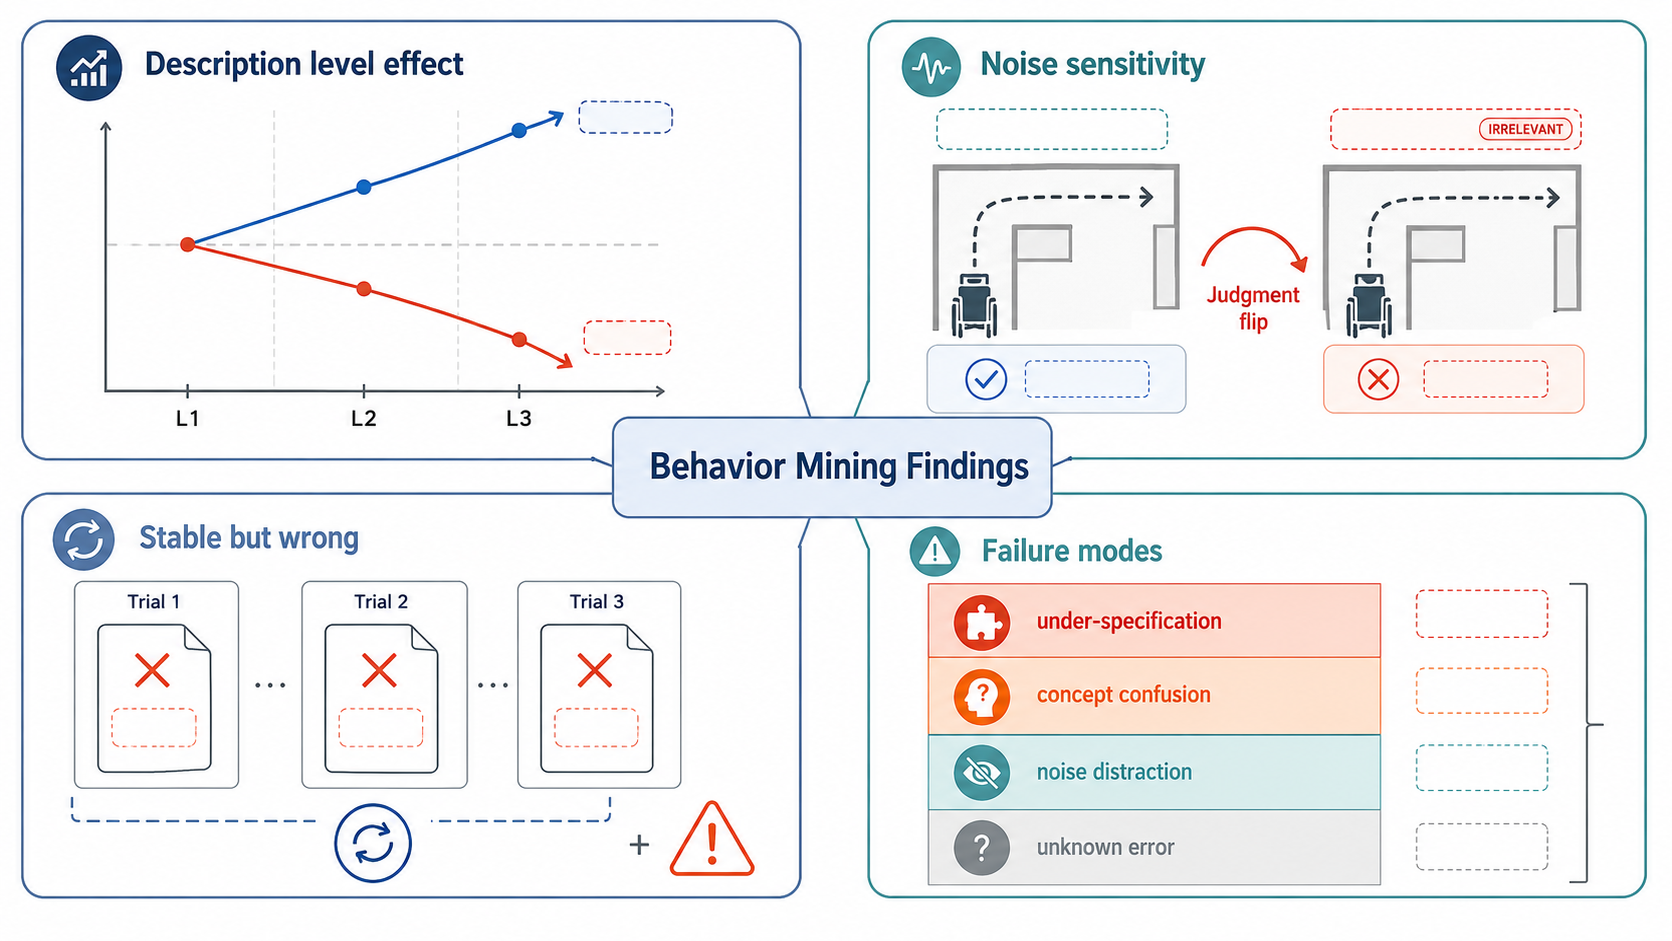
\includegraphics[width=0.94\textwidth]{figures/key_findings_summary.png}
\caption{核心规律发现总览。四个面板分别对应描述层级效应、噪声敏感度、稳定错误和失效模式集中性。}
\label{fig:key-findings-summary}
\end{figure*}

\subsection{挖掘方法}

根据任务要求，本文的数据挖掘目标不是直接求解轮椅能否通过，而是把不同大语言模型对同一空间场景的判断过程作为行为数据来分析。因此，挖掘流程围绕四个问题展开：第一，描述方式从 L1 自然语言、L2 具体参数到 L3 数学建模时，模型判断是否保持一致；第二，加入光照、材质、噪声、情绪压力等无关信息后，模型是否发生逻辑偏移；第三，不同模型的认知边界能否按行为画像聚成若干类型；第四，错误回复能否被归纳为可解释的失效模式。表 \ref{tab:mining-methods} 在这一目标下汇总本文使用的主要方法。

所有方法都基于同一份行为特征长表 \path{data/processed/behavior_features_experiment.csv}。每一行对应一次模型回复，包含 \code{model}、\code{strategy}、\code{level}、\code{noise_label}、\code{repeat}、\code{ai_judgment}、\code{is_correct}、\code{error_category}、\code{reasoning_steps}、\code{has_formula}、\code{uses_coordinate} 和原始 \code{response} 等字段。这样，统计结果、聚类结果、关联规则和典型文本样本可以互相回溯，避免只给出孤立的平均分。

\begin{table*}[t]
\centering
\caption{本文使用的数据挖掘方法、任务映射与输出}
\label{tab:mining-methods}
\scriptsize
\begin{tabularx}{0.98\textwidth}{p{0.16\textwidth}p{0.19\textwidth}p{0.23\textwidth}Y}
\toprule
方法 & 对应任务要求 & 输入变量 & 输出与解释目标 \\
\midrule
覆盖率与数据审计 & 行为数据采集与标注 & \code{strategy}, \code{model}, \code{repeat}, \code{status} & 检查 1500 条 Prompt、12 个模型和 3 次重复的阶段性覆盖，确认当前 10{,}585 条成功回复可用于挖掘。\\
多维分组统计与热力图 & 认知层级对比 & \code{model}, \code{level}, \code{strategy}, \code{is_correct} & 计算模型、层级和生成策略维度下的准确率、公式率、坐标率和平均推理步数，识别形式化受益或数学化坍塌。\\
描述层级一致性挖掘 & 逻辑一致性探测 & 同一 \code{case_id}/\code{noise_label}/\code{repeat} 下的 L1--L3 回复 & 比较同一场景三种表述下的判断是否一致，定位“描述越数学越糊涂”的反常边界。\\
配对噪声翻转分析 & 描述敏感度挖掘 & 同一 \code{case_id}/\code{level}/\code{repeat} 下的 \code{none} 与噪声样本 & 计算无关描述导致的判断翻转率，衡量非因果信息对空间判断的干扰强度。\\
重复采样自一致性 & 逻辑稳定性探测 & 同一 \code{model} 和 \code{prompt_uid} 的 2--3 次回复 & 区分随机波动与稳定错误，发现“高自一致但低准确”的模型和样本。\\
失效模式分布分析 & 失效模式分类 & \code{error_category}, \code{model}, \code{level}, \code{noise_label} & 统计 \code{under_specification}、\code{concept_confusion}、\code{noise_distraction} 等错误外观，判断主要失败来源。\\
K-Means 模型画像聚类 & 模型认知边界聚类 & L1/L2/L3 准确率、层级一致性、噪声翻转率、公式率、坐标率 & 将模型聚成视觉直觉型、噪声敏感型、混合稳健型等行为类别。\\
FP-Growth 关联规则 & 深度规律发现 & \code{level}, \code{noise_label}, \code{criticality}, \code{ai_judgment}, \code{error_category} 等离散项 & 挖掘导致错误、不确定和特定失效模式的高支持、高置信组合。\\
决策树判别路径 & 可解释模型评估 & 几何余量、层级编码、是否临界、推理步数、公式/坐标特征 & 提取影响正确性的层级化判别条件，检查错误是否集中在临界余量和短推理链。\\
TF-IDF + K-Means 文本聚类 & 错误判例文本挖掘 & \code{error_category != none} 的原始回复文本 & 对错误回复做关键词聚类，归纳轮椅转弯空间逻辑中的典型盲区。\\
\bottomrule
\end{tabularx}
\end{table*}

\begin{figure*}[t]
\centering
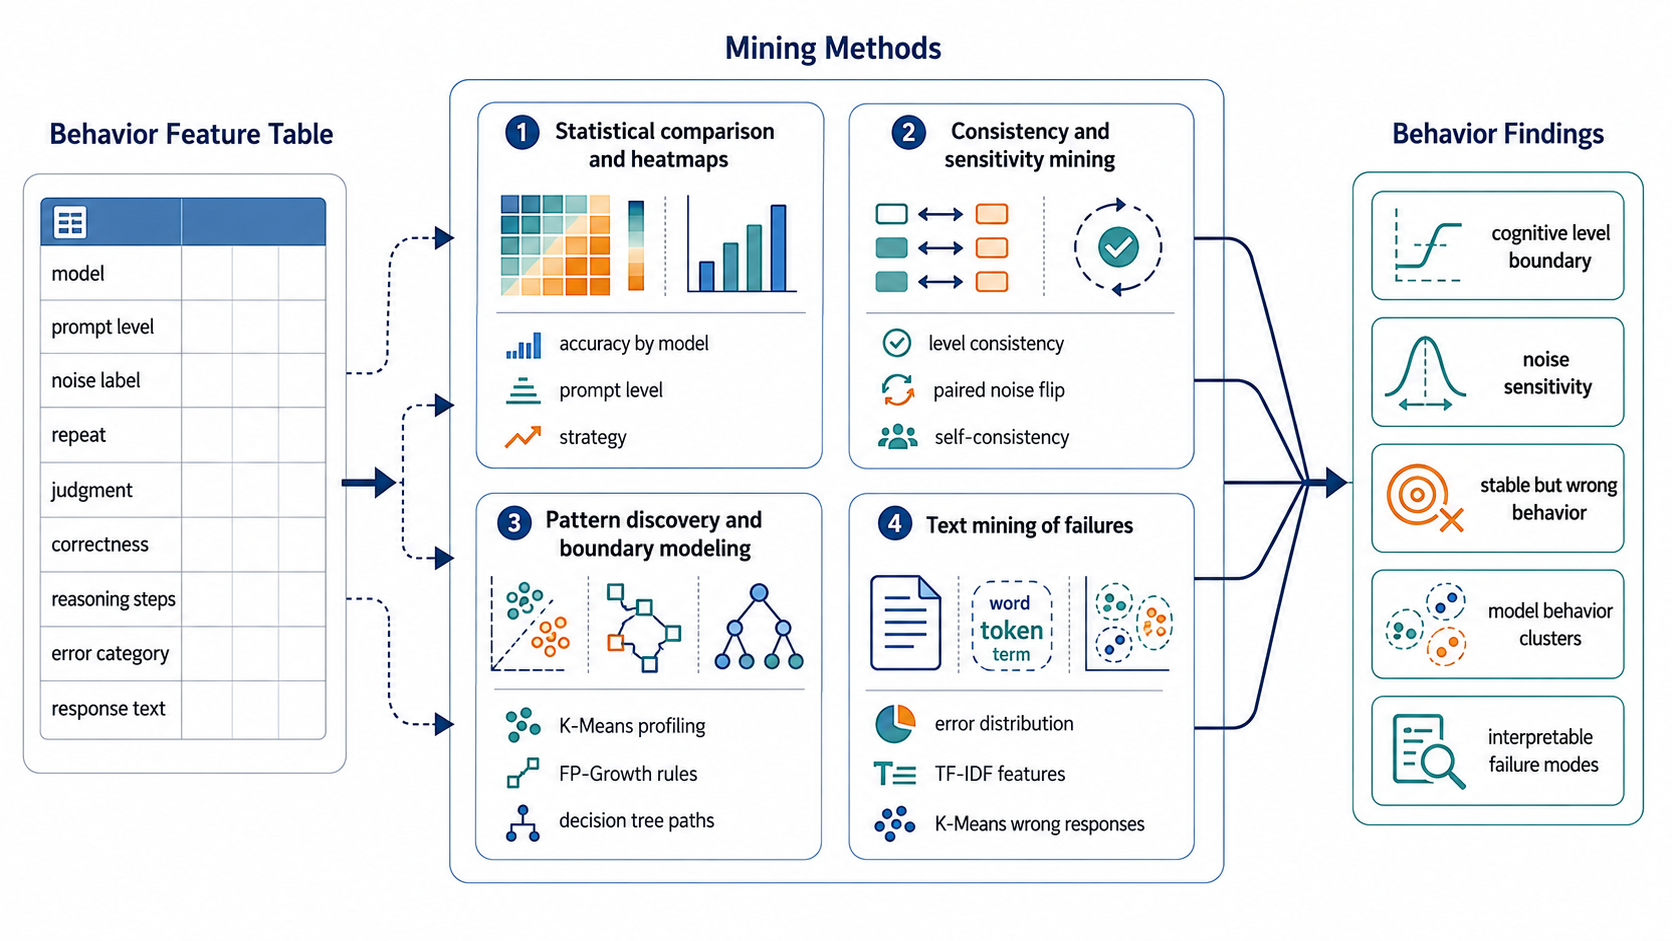
\includegraphics[width=0.92\textwidth]{figures/mining_method_principle.png}
\caption{数据挖掘方法原理图。行为特征长表同时流向几何余量风险、Prompt 策略效应、判断混淆矩阵、层级迁移路径、噪声关键词吸收、稳定错误案例库、聚类、关联规则、决策树和文本聚类等分析模块。}
\label{fig:mining-method-principle}
\end{figure*}

\subsubsection{分层统计与覆盖率审计}

在正式挖掘前，本文先进行覆盖率和质量审计。Prompt 主表固定为 5 类生成策略、3 个描述层级和 5 类扰动条件；回复表按 \code{strategy}、\code{model} 和 \code{repeat} 汇总 \code{observed_rows}、\code{success_rows}、\code{coverage_rate} 和 \code{success_rate}。这一步的目的不是得出模型能力结论，而是判断后续统计是否有足够样本支撑。例如，当前数据覆盖 9 个有成功样本的模型，但不同模型的回收量并不完全一致，因此论文在解释 DeepSeek-v4-pro 和 Kimi-K2-Thinking 等样本较少的模型时只把它们作为趋势观察，而不直接给出总体优劣排序。

在通过质量审计后，本文计算分组准确率
\[
A_{m,l}=\frac{1}{N_{m,l}}\sum_{i:\,model_i=m,\,level_i=l}\mathbf{1}(is\_correct_i),
\]
并同时保留 \code{formula_rate}、\code{coordinate_rate} 和 \code{avg_steps}。准确率热力图展示模型在 L1、L2、L3 三个层级下的变化，雷达图则把准确率、一致性和形式化行为放在同一坐标系中比较。这样可以回答任务要求中的“自然语言描述”和“形式化几何建模”接受度差异，而不是只报告一个总分。

\subsubsection{层级一致性与噪声敏感度}

层级一致性用于衡量同一空间场景在不同表达范式下是否保持相同判断。对同一 \code{model}、\code{case_id}、\code{noise_label} 和 \code{repeat}，若同时存在 L1、L2、L3 三条回复，记三个判断为 $y_1,y_2,y_3$，则一致性得分定义为
\[
C=\frac{\mathbf{1}(y_1=y_2)+\mathbf{1}(y_1=y_3)+\mathbf{1}(y_2=y_3)}{3}.
\]
$C=1$ 表示三种描述完全一致，$C=0$ 表示三对判断全部不一致。该指标直接对应任务要求中的“逻辑一致性探测”，可以发现模型是否在参数更精确时反而改变结论。

噪声敏感度采用配对翻转设计。对同一个 \code{case_id}、\code{level} 和 \code{repeat}，以 \code{noise_label=none} 的回复作为基线，再与光照、材质颜色、环境噪声和情绪压力等无关扰动版本配对。若两者的 \code{ai_judgment} 不同，则记为一次翻转，模型 $m$ 在噪声类型 $n$ 下的翻转率为
\[
F_{m,n}=\frac{1}{P_{m,n}}\sum_{p=1}^{P_{m,n}}\mathbf{1}(y^{noise}_{p}\neq y^{none}_{p}).
\]
由于几何参数和参考标签在配对样本中保持不变，翻转率可以更直接地解释为非因果文本线索对判断链条的干扰，而不是题目难度变化造成的差异。

\subsubsection{重复采样稳定性与稳定错误}

为了区分”模型随机摇摆”和”模型稳定走错”，本文借鉴自一致性思路\cite{wang2023self}，进一步分析同一 \code{model} 与 \code{prompt_uid} 下的 2--3 次重复采样。若同组回复的 \code{ai_judgment} 只有一个取值，则记为完全自一致；若出现两个或三个取值，则说明同一 Prompt 下存在采样波动。模型级自一致性定义为完全一致组数占全部可比较组数的比例：
\[
S_m=\frac{\#\{\text{fully consistent groups of }m\}}{\#\{\text{groups of }m\text{ with at least two repeats}\}}.
\]
这一指标与组均准确率联合解释：高 $S_m$ 且高准确说明模型稳定可靠；低 $S_m$ 说明模型对同一输入不稳定；高 $S_m$ 但低准确则是更危险的“稳定错误”，即模型虽然多次给出相同判断，却持续偏离参考标签。

\subsubsection{模型画像聚类与失效文本挖掘}

模型认知边界聚类把每个模型压缩为七维画像：L1、L2、L3 准确率、层级一致性、平均噪声翻转率、公式率和坐标率。由于这些指标量纲不同，先使用标准化处理，再用 K-Means 进行聚类。聚类结果不被解释为模型的永久标签，而是解释为该轮椅转弯任务下的行为类型，例如视觉直觉型、噪声敏感型和混合稳健型。该方法对应任务要求中的“模型认知边界聚类”，用于回答不同模型在什么表达精度和扰动条件下发生逻辑坍塌。

错误文本挖掘只使用 \code{error_category != none} 的回复。首先通过规则化特征把错误样本分成 \code{under_specification}、\code{concept_confusion}、\code{noise_distraction} 和 \code{unknown_error}；然后对原始回复做中文/英文 token 抽取、TF-IDF 向量化和 K-Means 聚类，输出每个簇的规模、关键词、主导模型、主导失效模式和样例文本。前者给出结构化错误分布，后者保留自然语言中的具体盲区，能够解释模型是把旋转包络、最小转弯半径和平台进深混淆，还是被“缺少尺寸”的模板化拒答牵引。

\subsubsection{关联规则与决策树解释}

关联规则挖掘把每条回复转换为 \code{key=value} 形式的事务项，例如 \code{level=L3}、\code{noise_label=lighting}、\code{ai_judgment=uncertain} 和 \code{error_category=under_specification}。本文使用 FP-Growth\cite{han2000mining} 搜索频繁项集（关联规则挖掘的经典形式化见 \citeauthor{agrawal1993mining}\cite{agrawal1993mining}），再用支持度、置信度和提升度筛选规则：
\[
\begin{aligned}
support(X\Rightarrow Y)&=P(X\cup Y),\\
confidence(X\Rightarrow Y)&=P(Y|X),\\
lift(X\Rightarrow Y)&=\frac{P(Y|X)}{P(Y)}.
\end{aligned}
\]
其中后件优先限制为 \code{is_correct}、\code{is_uncertain}、\code{ai_judgment} 或 \code{error_category}，使规则直接指向正确性、不确定性和失败类别。与热力图相比，关联规则更适合发现多个条件共同出现时的高置信行为模式。

决策树则以 \code{is_correct} 为目标变量，以 \code{level_code}、\code{has_noise}、\code{is_borderline}、\code{clearance_margin_cm}、\code{reasoning_steps}、\code{has_formula} 和 \code{uses_coordinate} 为输入特征，最大深度限制为 4，基于 scikit-learn 实现\cite{pedregosa2011scikit}。树模型的作用不是追求最高预测精度，而是导出可读的分裂路径，观察“临界余量很小”“推理步数过短”“进入 L3 但没有正确使用坐标”等条件如何共同指向错误判断。它与 FP-Growth 互补：前者给出连续/数值特征上的阈值路径，后者给出离散行为项之间的共现规则。

\subsection{几何余量与临界阈值深挖}

为了避免结论只停留在文本层面，本文进一步把 \code{clearance_margin_cm} 与 \code{criticality} 纳入分析，输出 \path{margin_risk_summary.csv}。该表按模型、临界类别和余量区间统计准确率、不确定率、概念混淆率、信息不足率和噪声牵引率。总体结果见表 \ref{tab:margin-risk-overall}。这里最重要的发现是：几何上“明显不能通过”的 narrow 样本反而更容易被模型答对，而 wide 样本并不天然简单。原因在于 narrow 样本的参考标签多为 \code{cannot_pass}，模型保守回答会偶然命中；wide 样本需要模型真正识别可通行余量，否则会被轮椅长度、转弯半径或安全风险联想拉向错误的 \code{cannot_pass}。

\begin{table}[t]
\centering
\caption{几何临界性与模型行为风险}
\label{tab:margin-risk-overall}
\scriptsize
\begin{tabular}{lrrrrr}
\toprule
类别 & 样本 & 平均余量 & 准确率 & 不确定 & 概念混淆 \\
\midrule
\code{narrow} & 2163 & -9.65 & 73.6\% & 26.4\% & 0.0\% \\
\code{borderline} & 5657 & 2.23 & 40.1\% & 38.7\% & 15.8\% \\
\code{wide} & 2765 & 18.24 & 34.8\% & 26.6\% & 30.5\% \\
\bottomrule
\end{tabular}
\end{table}

这个结果解释了为什么决策树把 \code{clearance_margin_cm <= 2.50} 放在根节点：临界余量不仅改变正确率，也改变错误形态。borderline 样本的信息不足率达到 38.7\%，说明模型面对边界样本时经常退回“不确定”；wide 样本的概念混淆率达到 30.5\%，说明模型即使面对可通行余量，也可能把通道净宽、最小转弯半径和轮椅长度错误地合并成过度保守结论。因此，本文的“认知边界”不是单个准确率，而是几何余量、表达层级和模型保守倾向共同形成的边界。

\subsection{Prompt 生成策略效应}

Prompt 主表不是随机堆题，而是由五类场景生成策略构成。新增的 \path{strategy_effect_summary.csv} 按 \code{strategy} 和 \code{level} 输出策略效应，表 \ref{tab:strategy-effect-overall} 给出策略层面的汇总。结果显示，\code{constraint_boundary_solver} 的总体准确率为 60.6\%，明显高于 baseline 的 30.8\%。这说明更清晰地围绕约束边界构造样本，能让模型更容易提取关键变量；而 baseline 虽然更接近日常问法，却更容易诱发直觉化、模板化或安全保守回答。

\begin{table*}[t]
\centering
\caption{Prompt 生成策略对模型行为的影响}
\label{tab:strategy-effect-overall}
\footnotesize
\begin{tabularx}{0.98\textwidth}{p{0.27\textwidth}rrrrrrr}
\toprule
生成策略 & 样本 & 准确率 & 不确定 & 公式率 & 坐标率 & 概念混淆 & 信息不足 \\
\midrule
\code{constraint_boundary_solver} & 2098 & 60.6\% & 31.3\% & 76.6\% & 22.6\% & 5.4\% & 31.3\% \\
\code{real_world_archetype_matrix} & 2088 & 49.0\% & 32.1\% & 77.2\% & 22.2\% & 14.6\% & 32.1\% \\
\code{dimensionless_ratio_design} & 2097 & 48.9\% & 31.0\% & 73.2\% & 23.5\% & 15.5\% & 31.0\% \\
\code{halton_space_filling} & 2058 & 39.3\% & 34.5\% & 72.5\% & 21.7\% & 20.1\% & 34.5\% \\
\code{baseline} & 2244 & 30.8\% & 35.9\% & 75.9\% & 22.5\% & 25.8\% & 35.9\% \\
\bottomrule
\end{tabularx}
\end{table*}

策略效应也说明，本文的数据集构造本身就是一项数据挖掘设计，而不是把同一问题重复问多次。baseline 用于检验口语直觉，dimensionless ratio 用于检验尺度无关判断，boundary solver 用于逼近临界边界，real-world archetype 用于模拟真实场景，Halton space filling 用于覆盖参数空间。不同策略下错误率和错误类别不同，后续模型比较必须控制策略条件，否则很容易把“题目生成方式造成的差异”误读成模型能力差异。

\subsection{判断混淆矩阵与安全方向}

总体准确率无法区分两种不同风险：把可通行样本误判为不可通行，和把不可通行样本误判为可通行。为此，本文新增 \path{judgment_confusion_matrix.csv}，按 \code{reference_judgment} 与 \code{ai_judgment} 建立混淆矩阵。表 \ref{tab:judgment-confusion-overall} 显示，参考标签为 \code{can_pass} 的 5370 条样本中，模型只有 21.4\% 明确回答可通过，41.3\% 错误回答不可通过，37.3\% 退回不确定；参考标签为 \code{cannot_pass} 的样本中，危险的误判可通过仅占 1.0\%，但仍有 28.6\% 被回答为不确定。

\begin{table}[t]
\centering
\caption{参考标签与模型最终判断的总体混淆矩阵}
\label{tab:judgment-confusion-overall}
\footnotesize
\begin{tabular}{llrr}
\toprule
参考标签 & 模型判断 & 数量 & 类内占比 \\
\midrule
\code{can_pass} & \code{can_pass} & 1150 & 21.4\% \\
\code{can_pass} & \code{cannot_pass} & 2219 & 41.3\% \\
\code{can_pass} & \code{uncertain} & 2001 & 37.3\% \\
\code{cannot_pass} & \code{can_pass} & 51 & 1.0\% \\
\code{cannot_pass} & \code{cannot_pass} & 3670 & 70.4\% \\
\code{cannot_pass} & \code{uncertain} & 1494 & 28.6\% \\
\bottomrule
\end{tabular}
\end{table}

这组结果表明，模型在本任务中最突出的偏差不是冒险放行，而是过度保守和拒答。对于真实无障碍安全评估，冒险放行的 51 例需要特别警惕；但从认知边界角度看，更大规模的现象是模型面对可通行样本时无法建立充分空间模型，转而把“轮椅较大”“转角紧凑”“安全风险”等一般性线索当成否定证据。因此，本文后续讨论中的“稳定错误”主要指稳定地把可通行样本判为不可通行或不确定。

\subsection{L1--L3 层级迁移路径}

层级一致性得分能说明模型是否变化，但不能说明变化方向。新增的 \path{level_transition_patterns.csv} 把同一 \code{case_id}/\code{noise_label}/\code{repeat} 下的 L1、L2、L3 判断串成路径，例如 \code{uncertain -> cannot_pass -> can_pass}。表 \ref{tab:transition-types} 将路径进一步归纳为五类。可以看到，数学化改善占 16.3\%，数学化坍塌占 24.3\%，后者规模更大。这直接支持“形式化描述不是单向增益”的结论。

\begin{table*}[t]
\centering
\caption{L1--L3 层级迁移路径类型}
\label{tab:transition-types}
\footnotesize
\begin{tabularx}{0.98\textwidth}{p{0.27\textwidth}rrrrrp{0.26\textwidth}}
\toprule
迁移类型 & 组数 & 占比 & L1 准确 & L2 准确 & L3 准确 & 解释 \\
\midrule
稳定或恢复正确 & 717 & 25.2\% & 100.0\% & 84.5\% & 100.0\% & L1 与 L3 都正确，中间层可能短暂波动。\\
数学化坍塌 & 691 & 24.3\% & 100.0\% & 17.8\% & 0.0\% & L1 正确，但进入 L3 后错误。\\
混合不稳定 & 506 & 17.8\% & 0.0\% & 19.6\% & 0.0\% & 三层之间存在局部变化，但没有形成 L3 改善。\\
稳定错误或拒答 & 465 & 16.4\% & 0.0\% & 0.0\% & 0.0\% & 三个层级均未命中参考标签。\\
数学化改善 & 462 & 16.3\% & 0.0\% & 68.8\% & 100.0\% & L1 错误或不确定，L3 后变正确。\\
\bottomrule
\end{tabularx}
\end{table*}

典型路径进一步揭示了模型差异。例如，GPT-4o 中大量样本从 \code{uncertain} 转向 \code{cannot_pass} 或 \code{can_pass}，说明形式化输入会显著改变其结论；Claude-Opus-4-6 与 GPT-4o-mini 中常见 \code{can_pass -> cannot_pass -> cannot_pass}，说明 L2/L3 参数化反而触发了过度保守；Gemini-3-Flash-Preview 的高频路径是 \code{uncertain -> uncertain -> uncertain}，说明它不是在层级之间摇摆，而是持续拒绝给出明确空间判断。路径分析比单一一致性分数更细，因为它能分辨“变好”“变坏”和“一直不行”三种完全不同的行为机制。

\subsection{噪声触发词复述与非因果线索吸收}

无关扰动是否影响模型，不能只看 Prompt 中有没有噪声，还要看模型是否把噪声词复述进自己的推理链。新增的 \path{noise_keyword_effect.csv} 使用 \code{noise_keyword_hit} 统计复述行为。总体上，未复述噪声关键词的样本为 5411 条，准确率 38.5\%；复述噪声关键词的样本为 3045 条，准确率 59.8\%。这说明“复述噪声”本身不必然降低准确率，一些较强模型会先复述背景再回到几何约束；但复述组的 \code{noise_distraction} 占比达到 8.8\%，显著高于未复述组的 0.7\%，说明真正发生噪声错误时，文本链条中通常能看到触发词痕迹。

\begin{table}[t]
\centering
\caption{噪声关键词复述与错误形态}
\label{tab:noise-keyword-effect}
\footnotesize
\begin{tabular}{lrrrr}
\toprule
是否复述 & 样本 & 准确率 & 不确定 & 噪声牵引 \\
\midrule
否 & 5411 & 38.5\% & 33.0\% & 0.7\% \\
是 & 3045 & 59.8\% & 30.7\% & 8.8\% \\
\midrule
\code{催促} & 179 & 52.0\% & 33.0\% & 15.1\% \\
\code{着急} & 616 & 56.2\% & 31.8\% & 10.7\% \\
\code{扶手} & 389 & 54.5\% & 35.2\% & 10.3\% \\
\bottomrule
\end{tabular}
\end{table}

这组结果的关键不在于“哪个词绝对最坏”，而在于建立了 Prompt 噪声、回复复述和错误类别之间的证据链。情绪压力类词汇如“催促”“着急”更容易把模型从几何判断拉向安全风险叙事；环境词如“噪声”“灯光”被频繁复述，但并不总是导致错误。由此可见，描述敏感度不是简单关键词过滤问题，而是模型是否把非因果线索纳入最终判定的问题。

\subsection{稳定错误案例库}

重复采样自一致性表明，有些模型并不是随机波动，而是稳定地走向同一个错误结论。本文新增 \path{stable_wrong_casebook.csv}，先识别同一 \code{model}/\code{prompt_uid} 下至少两次重复采样、且所有 \code{ai_judgment} 完全一致并全部错误的样本，再按错误类别分层保留代表案例。完整候选中，稳定错误主要来自 \code{under_specification}、\code{concept_confusion}、\code{noise_distraction} 和 \code{unknown_error}；导出的案例库每类保留 20 条，共 80 条，用于人工复核和论文案例解释。

\begin{table*}[t]
\centering
\caption{稳定错误案例库中的代表样本}
\label{tab:stable-wrong-casebook}
\scriptsize
\begin{tabularx}{0.98\textwidth}{p{0.16\textwidth}p{0.12\textwidth}p{0.12\textwidth}p{0.13\textwidth}p{0.12\textwidth}Y}
\toprule
错误类别 & 模型 & 场景 & 条件 & 稳定误判 & 证据解释 \\
\midrule
概念混淆 & Claude-Opus-4-6 & C003, L2 & baseline + 环境噪声，余量 8cm & \code{can_pass -> cannot_pass} & 三次重复均判为不可通过；回复把最小转弯半径和实际可用包络混为更保守的空间需求。\\
噪声牵引 & Claude-Sonnet-4-6-Thinking & C001, L2 & baseline + 环境噪声，余量 14cm & \code{can_pass -> cannot_pass} & 三次重复均判为不可通过；回复将 86cm 转弯半径扩大成约 172cm 的正方形需求，并叠加环境风险。\\
信息不足 & Kimi-K2-Thinking & C001, L1 & Halton + 材质颜色，余量 22cm & \code{can_pass -> uncertain} & 三次重复均为不确定；口语描述中的“宽裕”没有被转化为可用余量，而是触发缺少精确尺寸的拒答。\\
未知错误 & GPT-4o-mini & C004, L1 & Halton + 情绪压力，余量 6cm & \code{can_pass -> cannot_pass} & 三次重复均判为不可通过；回复只给出一般风险叙述，没有明确使用已知几何变量。\\
\bottomrule
\end{tabularx}
\end{table*}

案例库的意义在于把统计结论落回原始文本。表 \ref{tab:stable-wrong-casebook} 中的四类样本分别对应四种错误机制：把半径、宽度和平台进深混在一起；把无关环境风险纳入结论；把可用余量视为信息不足；以及没有可归因关键词但仍稳定保守。它们说明，模型失效不是单纯“答错”，而是具有可重复的文本外观和条件触发结构。

\subsection{描述层级：数学化并不稳定提升准确率}

图 \ref{fig:main-accuracy-radar} 左侧展示不同模型在 L1、L2、L3 下的准确率。结果显示，形式化描述对模型的作用高度分化。GPT-4o 从 L1 的 8.2\% 提升到 L3 的 59.2\%，DeepSeek-v4-pro 从 53.1\% 提升到 75.0\%，Kimi-K2-Thinking 从 85.5\% 提升到 94.4\%。这类模型在更明确的几何约束下更容易给出与参考边界一致的判断。

相反，Claude-Sonnet-4-6-Thinking 从 L1 的 47.4\% 下降到 L3 的 4.0\%，GPT-5.5 从 67.5\% 下降到 39.5\%，Claude-Opus-4-6 从 72.3\% 下降到 52.8\%，GPT-4o-mini 从 67.9\% 下降到 48.9\%。这说明“描述越数学，模型越可靠”并不是普遍规律；部分模型在看到坐标系、旋转包络和形式化判据后，会生成更长但更偏离的推理链。

\begin{figure*}[t]
\centering

\includegraphics[width=0.48\textwidth]{figures/accuracy_heatmap.png}\hfill

\includegraphics[width=0.48\textwidth]{figures/model_radar.png}
\caption{模型在不同描述层级下的准确率热力图与认知特征雷达图。}
\label{fig:main-accuracy-radar}
\end{figure*}

\begin{table*}[t]
\centering
\caption{描述层级变化下的模型认知边界}
\label{tab:cognitive-boundary}
\footnotesize
\begin{tabularx}{0.98\textwidth}{p{0.25\textwidth}rrrrp{0.22\textwidth}Y}
\toprule
模型 & L1 & L2 & L3 & L3-L1 & 类型 & 主要边界 \\
\midrule
\path{gpt-4o} & 8.2\% & 45.2\% & 59.2\% & +50.9 & 形式化受益型 & 自然语言层过度保守，进入 L2/L3 后才开始利用几何约束。\\
\path{deepseek-v4-pro} & 53.1\% & 66.7\% & 75.0\% & +21.9 & 形式化受益型 & 样本覆盖较少，但参数化表达明显优于口语描述。\\
\path{Kimi-K2-Thinking} & 85.5\% & 90.0\% & 94.4\% & +9.0 & 高准确稀疏型 & 当前成功样本少，需要谨慎解释，但已有样本中 L3 最稳。\\
\path{grok-4} & 65.9\% & 46.0\% & 57.0\% & -8.9 & 噪声敏感型 & L2 参数描述和无关噪声会同时拉低稳定性。\\
\path{gemini-3-flash-preview} & 31.9\% & 19.5\% & 16.7\% & -15.2 & 视觉直觉型 & 整体准确率较低，形式化表达没有带来收益。\\
\path{gpt-4o-mini} & 67.9\% & 48.7\% & 48.9\% & -19.0 & 视觉直觉型 & L1 表现最好，进入参数层后更容易混淆保守边界。\\
\path{claude-opus-4-6} & 72.3\% & 51.4\% & 52.8\% & -19.5 & 视觉直觉型 & 公式率很高，但 L2/L3 的准确率和一致性下降。\\
\path{gpt-5.5} & 67.5\% & 42.0\% & 39.5\% & -28.0 & 噪声敏感型 & 形式化与噪声共同诱发判断漂移。\\
\path{claude-sonnet-4-6-thinking} & 47.4\% & 34.4\% & 4.0\% & -43.3 & 数学化坍塌型 & L3 下公式率和推理步数同时下降，出现明显逻辑坍塌。\\
\bottomrule
\end{tabularx}
\end{table*}

\subsection{噪声敏感度：非因果信息会改变空间判断}

无关扰动不改变几何参数和参考标签，但会显著改变部分模型的最终判断。图 \ref{fig:main-noise-cluster} 左侧给出各干扰类型下的翻转率。最极端的例子是 Kimi-K2-Thinking 在 \code{emotional_pressure} 下翻转率达到 67.7\%（31 个样本）；DeepSeek-v4-pro 在 \code{lighting}、\code{material_color}、\code{ambient_noise} 和 \code{emotional_pressure} 下的翻转率均接近或超过 48\%；GPT-5.5 在 \code{emotional_pressure} 下翻转率为 44.3\%；Grok-4 在 \code{ambient_noise} 下为 36.3\%；Claude-Sonnet-4-6-Thinking 在 \code{material_color} 下为 36.4\%。

这类现象说明，模型并不总是先抽取几何变量再稳定推理。它们会把”灯光偏暗””有人催促””环境嘈杂””扶手颜色”等非因果线索错误地并入风险判断，进而从几何可通行切换到安全保守或不确定回答。这与推理链不忠实（unfaithful CoT）现象高度一致——模型表面给出推理步骤，实则受隐性偏置驱动\cite{turpin2023language}。输入格式与上下文敏感性在提示工程文献中也有类似记录\cite{lu2022fantastically,zhao2021calibrate}。按任务定义，这正是噪声诱发的逻辑偏移。

\begin{figure*}[t]
\centering
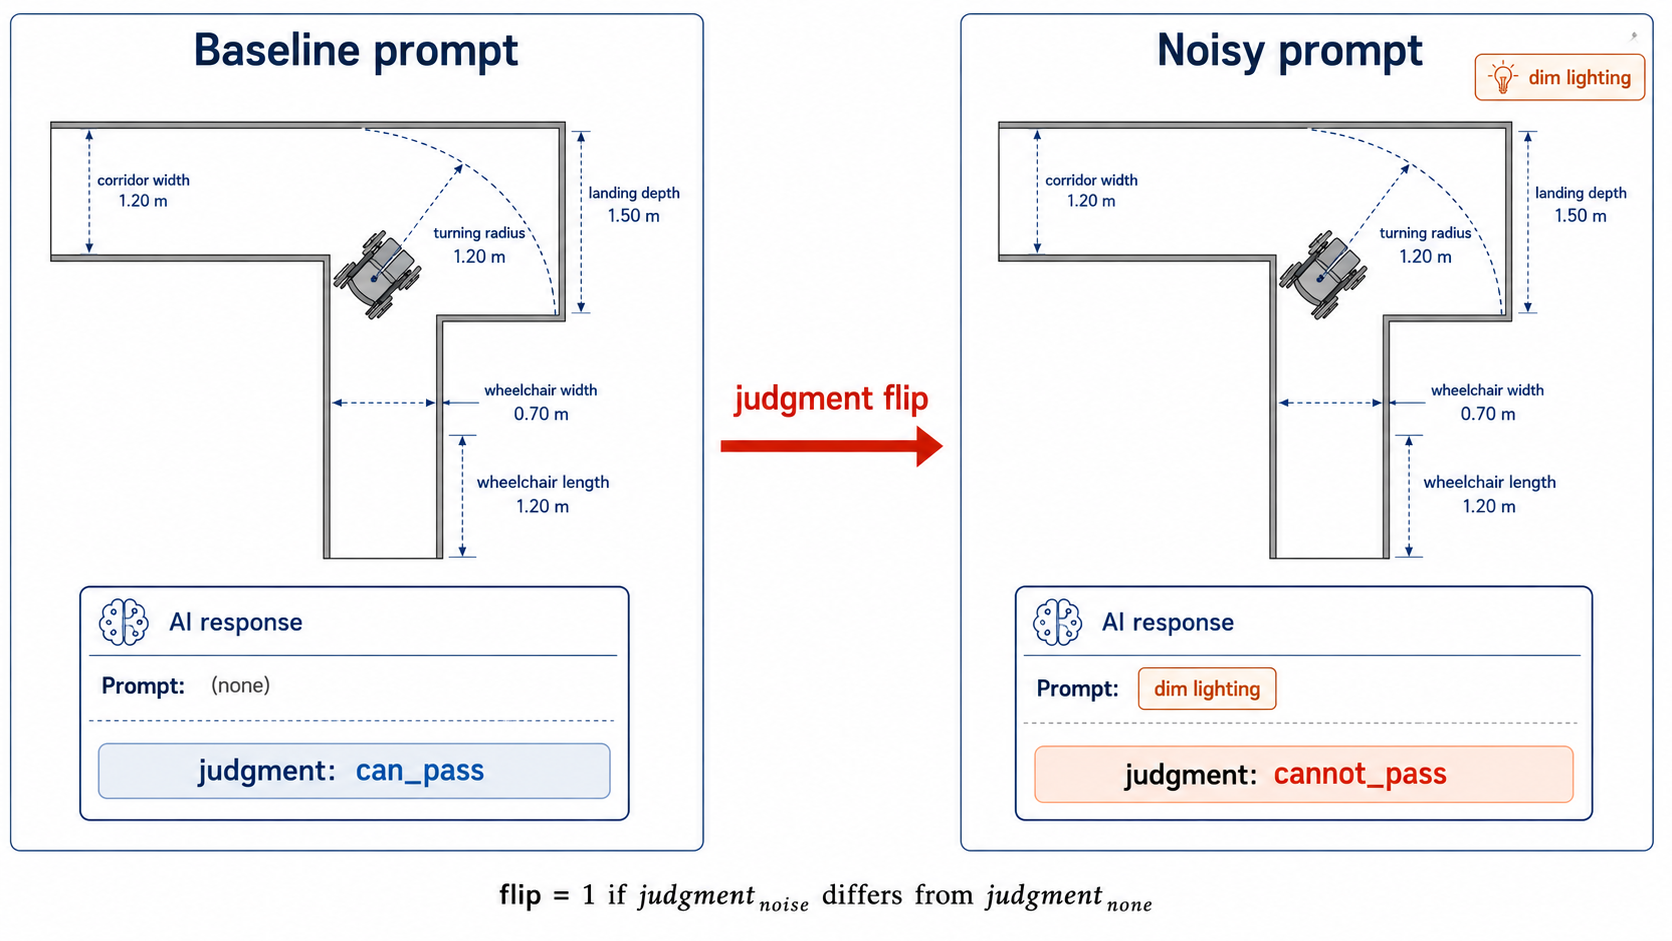
\includegraphics[width=0.92\textwidth]{figures/schema_noise_flip_pair.png}
\caption{非因果扰动导致判断翻转的配对样本示意。同一几何参数和参考标签保持不变，只改变背景噪声描述；若模型最终判断发生变化，则记为一次噪声翻转。}
\label{fig:noise-flip-pair-schema}
\end{figure*}

\begin{figure*}[t]
\centering

\includegraphics[width=0.48\textwidth]{figures/noise_flip_rate.png}\hfill

\includegraphics[width=0.48\textwidth]{figures/cluster_map.png}
\caption{无关扰动导致的判断翻转率与模型认知边界聚类视图。}
\label{fig:main-noise-cluster}
\end{figure*}

\begin{table}[t]
\centering
\caption{噪声翻转率最高的模型--扰动组合}
\label{tab:noise-top}
\footnotesize
\begin{tabularx}{\columnwidth}{@{}p{0.42\columnwidth}p{0.20\columnwidth}rr@{}}
\toprule
模型 & 扰动 & 翻转率 & 样本 \\
\midrule
\path{Kimi-K2-Thinking} & 情绪压力 & 67.7\% & 31\\
\path{deepseek-v4-pro} & 光照 & 50.0\% & 42\\
\path{deepseek-v4-pro} & 材料颜色 & 49.0\% & 51\\
\path{deepseek-v4-pro} & 情绪压力 & 48.7\% & 39\\
\path{gpt-5.5} & 情绪压力 & 44.3\% & 255\\
\path{claude-sonnet-4-6-thinking} & 材料颜色 & 36.4\% & 269\\
\bottomrule
\end{tabularx}
\end{table}

\subsection{一致性：存在“稳定地错”的模型}

层级一致性比较同一场景在 L1、L2、L3 三种表述中的判断是否一致。GPT-4o 的平均层级一致性只有 29.2\%，说明它在表达方式变化时经常改变结论；Grok-4 为 49.5\%，GPT-5.5 为 56.3\%，Claude-Opus-4-6 为 60.0\%。这类结果与准确率共同表明：模型能力边界不只由几何难度决定，也由题干的语言组织方式决定。

重复采样自一致性进一步揭示另一类风险。Claude-Opus-4-6、GPT-4o、Gemini-3-Flash-Preview 的三次采样自一致性分别为 85.0\%、83.8\%、83.8\%，但其中 GPT-4o 的组均准确率只有 37.6\%，Gemini-3-Flash-Preview 只有 23.6\%。也就是说，模型有时不是随机摇摆，而是稳定沿着错误路径作答。对于空间安全类问题，这种“自信但错误”比偶然波动更值得警惕。

\begin{figure*}[t]
\centering
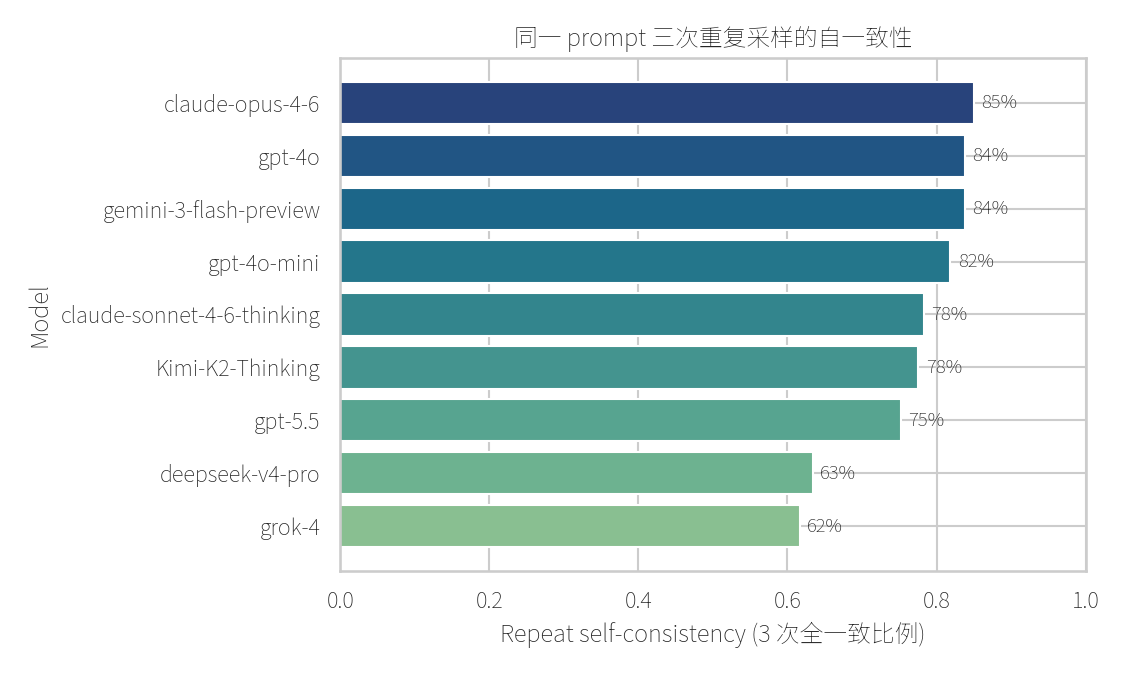
\includegraphics[width=0.48\textwidth]{figures/self_consistency_by_model.png}\hfill
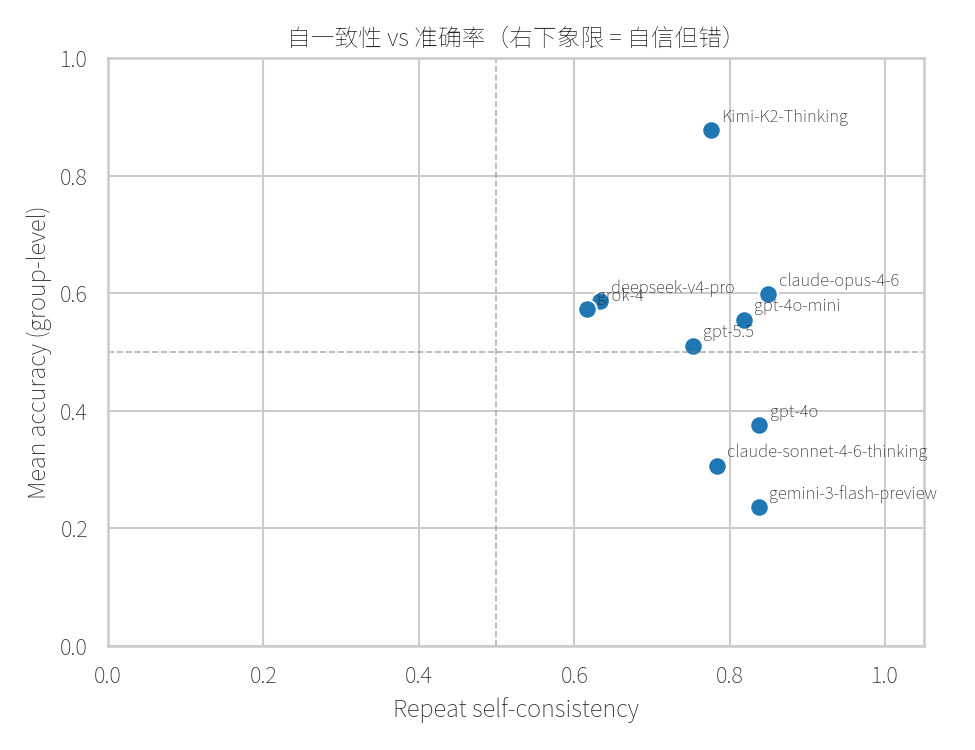
\includegraphics[width=0.48\textwidth]{figures/self_consistency_vs_accuracy.png}
\caption{重复采样自一致性与准确率关系。右下区域表示高自一致但低准确的稳定错误。}
\label{fig:main-self-consistency}
\end{figure*}

\begin{table}[t]
\centering
\caption{重复采样自一致性结果}
\label{tab:self-consistency-main}
\footnotesize
\begin{tabularx}{\columnwidth}{p{0.46\columnwidth}rrr}
\toprule
模型 & 组数 & 自一致性 & 均准确率 \\
\midrule
\path{claude-opus-4-6} & 426 & 85.0\% & 59.8\%\\
\path{gpt-4o} & 600 & 83.8\% & 37.6\%\\
\path{gemini-3-flash-preview} & 444 & 83.8\% & 23.6\%\\
\path{gpt-4o-mini} & 600 & 81.8\% & 55.5\%\\
\path{claude-sonnet-4-6-thinking} & 429 & 78.3\% & 30.7\%\\
\path{gpt-5.5} & 440 & 75.2\% & 51.1\%\\
\path{grok-4} & 404 & 61.6\% & 57.3\%\\
\bottomrule
\end{tabularx}
\end{table}

\subsection{模型认知边界聚类}

本文用 L1/L2/L3 准确率、层级一致性、平均噪声翻转率、公式率和坐标系使用率构成模型画像，并对有完整 L1--L3 配对统计的模型做标准化 K-Means 聚类。聚类结果显示，GPT-4o 单独表现为“混合稳健型”：噪声翻转率较低，但层级一致性最低，说明它不是被无关背景严重牵引，而是对表达范式非常敏感。Claude-Opus-4-6、Gemini-3-Flash-Preview 和 GPT-4o-mini 更接近“视觉直觉型”，共同特征是 L1 表现相对更好，L3 不一定带来收益。Claude-Sonnet-4-6-Thinking、GPT-5.5、Grok-4 和 DeepSeek-v4-pro 被归入“噪声敏感型”，主要边界出现在无关描述扰动下。

这种聚类并不是给模型贴固定标签，而是给出本任务下的行为画像。尤其要注意，DeepSeek-v4-pro 和 Kimi-K2-Thinking 的成功样本数少于其他主力模型，因此更适合用于观察趋势，不宜单独作为总体优劣结论。

\begin{figure*}[t]
\centering
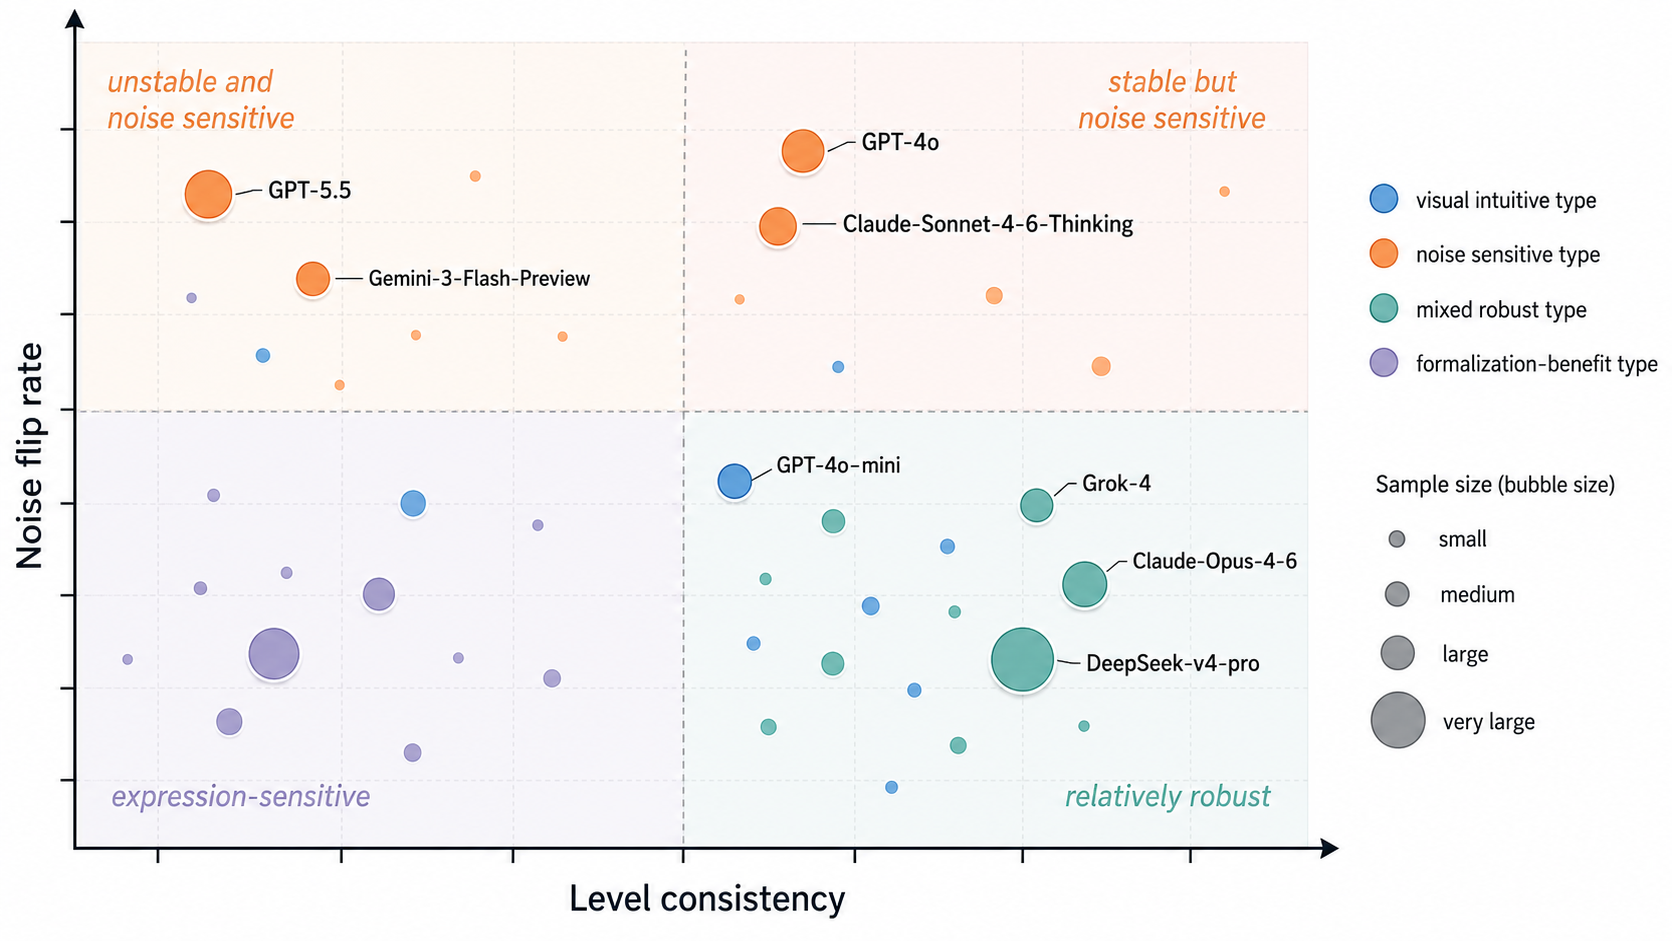
\includegraphics[width=0.92\textwidth]{figures/schema_cognitive_boundary_quadrants.png}
\caption{模型认知边界二维象限图。横轴表示描述层级一致性，纵轴表示噪声翻转率；点的位置、大小和颜色共同呈现模型在本任务下的稳定性、扰动敏感度和聚类类型。}
\label{fig:cognitive-boundary-quadrants}
\end{figure*}

\subsection{失效模式与错误文本聚类}

当前 10{,}585 条回复中有 5{,}765 条与参考标签不一致。错误类别分布为：\code{under_specification} 3{,}495 条，\code{concept_confusion} 1{,}734 条，\code{noise_distraction} 313 条，\code{unknown_error} 223 条。这类失效模式与文献中对 LLM 幻觉的分类体系相呼应\cite{ji2023survey}：最大的一类错误不是算术错误，而是模型声称”缺少关键尺寸，无法判断”，即使题干在 L2 或 L3 中已经给出足够参数。第二大类是概念混淆，常见表现是把轮椅长度直接与平台进深比较，或者把最小转弯半径、旋转包络和通道净宽混为同一约束。

TF-IDF + K-Means 对错误回复进一步分成四个文本簇。最大簇包含 1{,}976 条，关键词集中在“轮椅、cm、转弯、平台、通道、旋转、包络、半径”，主导模型为 GPT-4o，主导失效模式是 \code{concept_confusion}。第二簇包含 1{,}688 条，关键词集中在“转角、空间、可能、宽度”等模糊词，主导失效模式是 \code{under_specification}。第三簇包含 1{,}315 条，主要是拒答或无法讨论式回复；第四簇包含 236 条，常见英文安全策略或 prompt-injection 相关表述，主导失效模式为 \code{unknown_error}。这些簇说明错误并非均匀分布，而是集中在若干可解释的文本行为模式中。

\begin{table*}[t]
\centering
\caption{典型错误案例、触发条件与挖掘证据}
\label{tab:typical-error-cases}
\footnotesize
\renewcommand{\arraystretch}{1.16}
\begin{tabularx}{0.98\textwidth}{p{0.12\textwidth}p{0.40\textwidth}Y}
\toprule
失效类别 & 触发条件与典型回复 & 错误机制与挖掘证据 \\
\midrule
信息不足 &
\textbf{条件：}GPT-4o，C001，L1，无遮挡，参考标签为 \code{can_pass}。\par
\textbf{片段：}“没有提供具体空间尺寸、转弯半径或操控性能，无法得出明确结论。” &
\textbf{机制：}把自然语言层的主观描述视为不可判定，退回信息不足模板。\par
\textbf{证据：}该类共 3{,}495 条，占全部错误样本 60.6\%；不确定判断与该类一一对应。\\
\midrule
概念混淆 &
\textbf{条件：}GPT-4o，C001，L2，无遮挡，参考标签为 \code{can_pass}。\par
\textbf{片段：}“轮椅长度 105 cm 大于平台进深 100 cm，转弯时可能超出边界。” &
\textbf{机制：}把车体长度、平台进深、转弯半径和旋转包络混作单一约束。\par
\textbf{证据：}FP-Growth 规则显示，错误的“不能通过”且未命中噪声词时，87.9\% 指向概念混淆。\\
\midrule
噪声牵引 &
\textbf{条件：}GPT-4o，C001，L2，情绪压力，参考标签为 \code{can_pass}。\par
\textbf{片段：}“旁观者催促不改变物理限制，但最终判断：不能通过。” &
\textbf{机制：}表面声明噪声无关，实际判断仍被风险语境推向保守结论。\par
\textbf{证据：}噪声翻转分析显示，情绪压力、光照和材质颜色可使部分模型翻转率超过 40\%。\\
\midrule
未知错误 &
\textbf{条件：}GPT-4o-mini，C003，L1，无遮挡，参考标签为 \code{can_pass}。\par
\textbf{片段：}“转角紧凑且轮椅宽度较大，完成 90 度转弯的可能性较低。” &
\textbf{机制：}未形成明确几何比较，也无法归入信息不足或概念混淆。\par
\textbf{证据：}文本聚类中存在 236 条安全策略、拒答或泛化判断样本，主导类别为未知错误。\\
\bottomrule
\end{tabularx}
\end{table*}

\begin{figure*}[t]
\centering
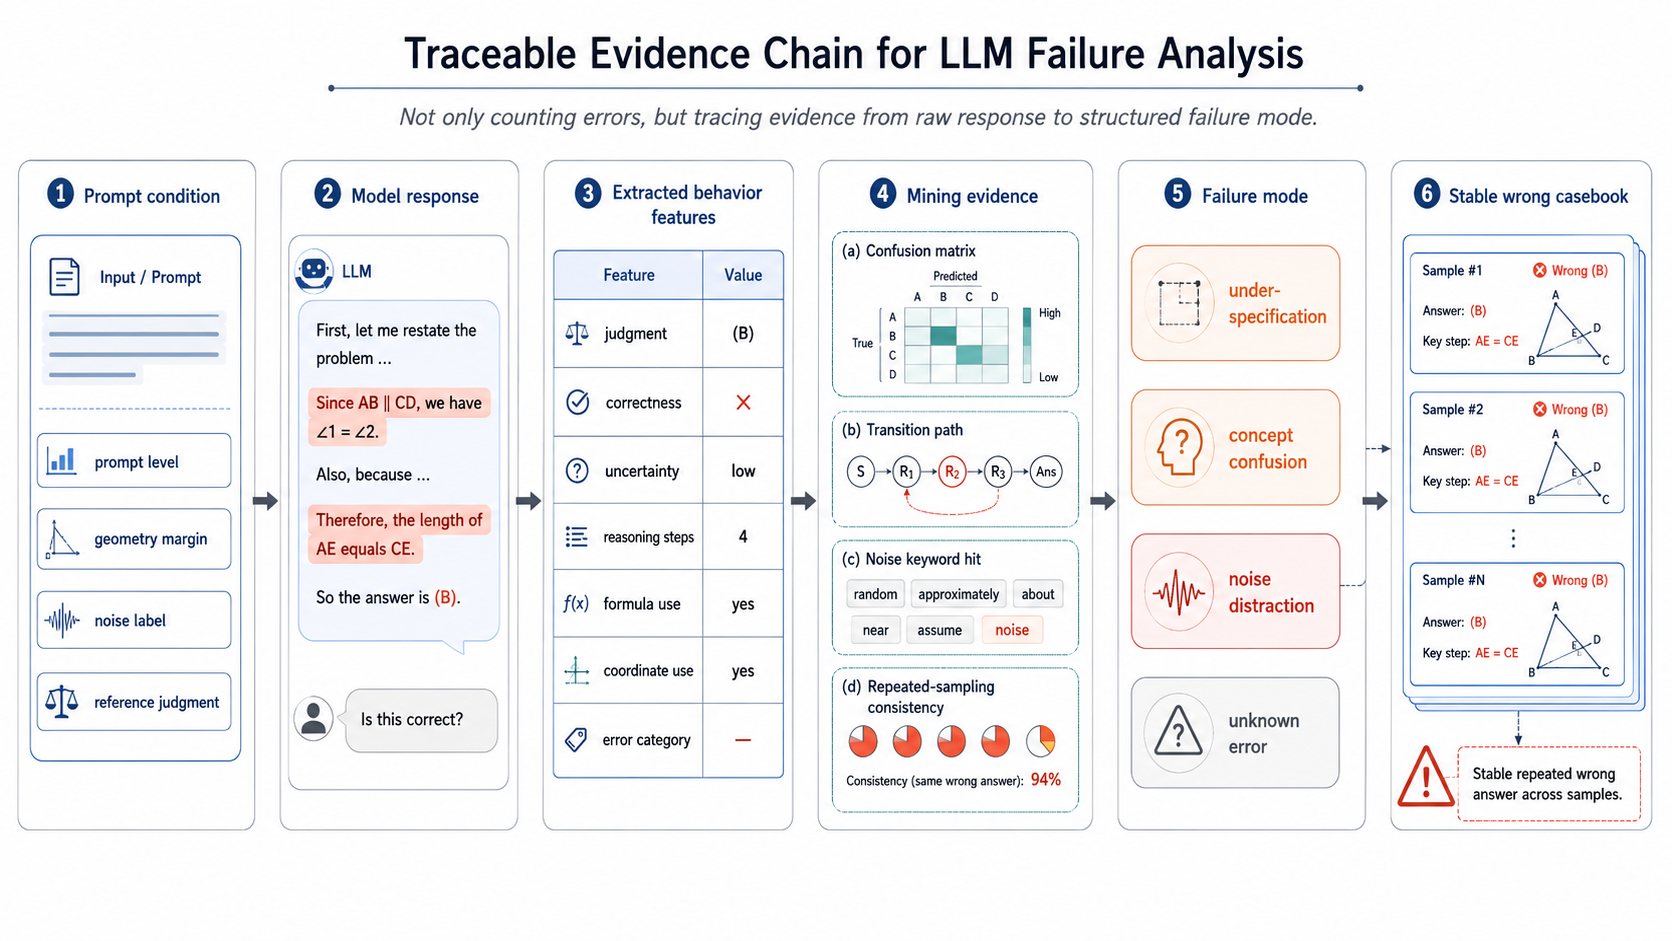
\includegraphics[width=0.92\textwidth]{figures/failure_evidence_chain.png}
\caption{错误机制证据链图。单个失效案例从 Prompt 条件、模型原始回复、结构化行为特征、挖掘指标到失效模式和稳定错误案例库逐层回溯，说明本文不是只统计错误数量，而是建立可解释的证据链。}
\label{fig:failure-evidence-chain}
\end{figure*}

\begin{figure*}[t]
\centering

\includegraphics[width=0.48\textwidth]{figures/failure_modes.png}\hfill
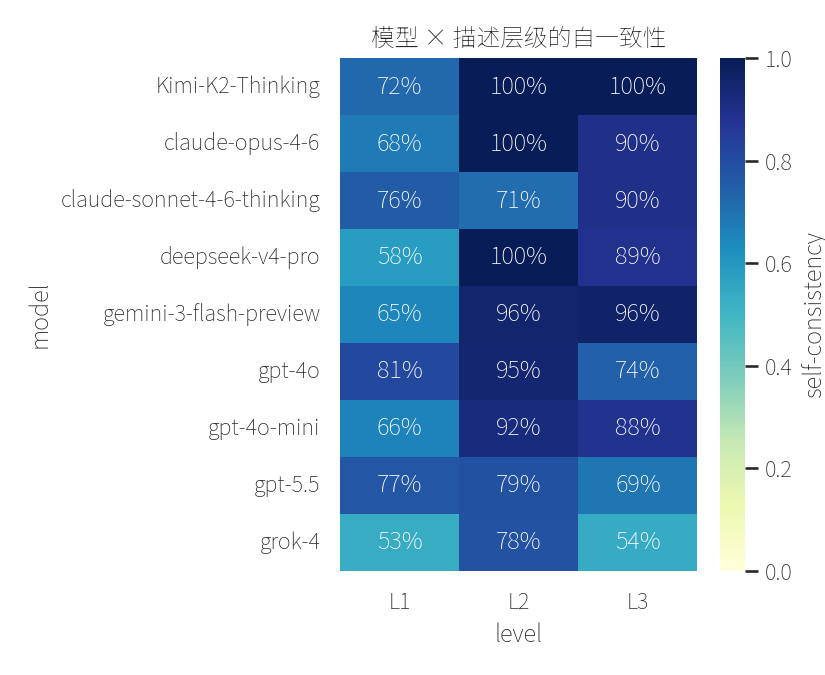
\includegraphics[width=0.48\textwidth]{figures/self_consistency_heatmap_level.png}
\caption{错误样本失效模式与不同层级下的重复采样自一致性。}
\label{fig:main-failure-self}
\end{figure*}

\subsection{关联规则与决策树发现}

FP-Growth 使用最小支持度 0.10、最小置信度 0.60，对行为特征离散项进行关联规则挖掘。结果中最强的失效规则之一为
\begin{center}
\footnotesize
\begin{tabular}{@{}l@{}}
\{\code{ai_judgment=cannot_pass}, \code{is_correct=0}\}\\
\quad + \{\code{noise_keyword_hit=none}\}\\
\quad $\Rightarrow$ \{\code{error_category=concept_confusion}\}.
\end{tabular}
\end{center}
置信度为 87.9\%，lift 为 5.37。这说明在没有复述噪声关键词、但明确给出错误“不通过”结论的样本中，错误往往来自几何概念混淆，而不是被背景噪声拉偏。另一条高支持规则是 \code{ai_judgment=uncertain} $\Rightarrow$ \code{error_category=under_specification}，支持度和置信度均为 33.0\% 与 100.0\%。该规则一方面反映了标注逻辑，另一方面也说明“不确定”是本任务最主要的失败外观。

决策树以 \code{is_correct} 为目标变量，最大深度为 4。根节点首先选择 \code{clearance_margin_cm <= 2.50}，说明临界余量仍是解释模型正确性的首要变量；随后分裂主要落在 \code{reasoning_steps}、\code{level_code}、\code{is_borderline} 和 \code{uses_coordinate} 上。可解释路径显示，在极小余量且推理步数不超过 1.5 的样本中，模型更容易直接给出错误或不完整判断；在非临界 L1 样本中，推理步数超过 1.5 时更容易预测为正确。这与前面的发现一致：模型不是单纯需要更长回复，而是需要在正确抽取几何变量后再推理\cite{wei2022chain,kojima2022large}；没有变量抽取的短答和错误形式化都会导致逻辑坍塌。

\section{结论与讨论}

本文把“轮椅能否在楼梯转角处完成 $90^\circ$ 转弯”转化为大语言模型行为数据挖掘任务，完成了 Prompt 矩阵构造、API 行为采集、结构化特征抽取、覆盖率审计、多维分组统计、准确率热力图、几何余量风险分析、Prompt 策略效应分析、判断混淆矩阵、层级迁移路径、噪声关键词复述分析、稳定错误案例库、层级一致性、噪声翻转、重复采样自一致性、失效模式分布、K-Means 模型画像聚类、FP-Growth 关联规则、决策树判别路径和 TF-IDF 错误文本聚类分析。结果表明，LLM 的空间推理边界具有明显的模型依赖性：有些模型受益于形式化描述，有些模型在 L3 下反而坍塌；有些模型对情绪、光照、噪声等非因果线索高度敏感；还有些模型虽然三次采样稳定，却稳定输出错误结论。值得注意的是，即便是 GPT-4 级别的模型在早期评测中就被观察到具有有限但值得研究的空间推理迹象\cite{bubeck2023sparks}，本文的大规模对比实验进一步揭示了这类能力在严格空间约束下的系统性局限。

从课程交付角度看，本文已经形成完整闭环：\path{data/experiment_prompts.csv} 给出多层级 Prompt 数据集，\path{data/raw/model_responses_experiment.csv} 保留原始 AI 行为，\path{data/processed/behavior_features_experiment.csv} 提供结构化行为特征，\path{scripts/} 和 \path{src/spatial_llm_mining/} 提供采集、清洗、挖掘和可视化代码，\path{outputs_experiment/} 保存可复查的统计表、图像和自动生成发现，最终 PDF 报告则把任务定义、方法、结果、局限和附录证据串联起来。新增的六张表 \path{margin_risk_summary.csv}、\path{strategy_effect_summary.csv}、\path{judgment_confusion_matrix.csv}、\path{level_transition_patterns.csv}、\path{noise_keyword_effect.csv} 与 \path{stable_wrong_casebook.csv} 进一步把工作量落实为可复查的数据资产。因此，本文的交付物不只是单篇分析文字，而是一套可复现的 AI 行为空间推理数据挖掘流程。

本研究的限制也需要明确。现场补充图显示，轮椅实际可占用区域是红线围出的不规则多边形，右上角斜边会改变旋转包络；因此，本文统计中的参考标签只能视为大规模行为挖掘的简化代理，不能替代真实无障碍规范、动力学仿真或现场安全评估。当前成功样本来自分批 API 快照，9 个模型的覆盖率并不完全一致，而且这些回复是在代理几何 Prompt 下采集的；若要直接回答现场图中的通行问题，应使用多边形 $\Omega$ 重新构造 Prompt 并重采模型回复。即便如此，10{,}585 条回复已经足以支持任务要求中的核心交付：结构化 AI 行为数据集、自动化评测与清洗代码，以及覆盖层级一致性、噪声敏感度、认知边界聚类和失效模式挖掘的 PDF 报告。
